% ---------
% RESULTATS
% ---------

% Defining TOC's sections before content
\section{Résultats}

\begin{frame}
    \begin{center}
    \vspace{0.5cm}
        \boxed{
        Résultats
        }
    \end{center}
\end{frame}

\begin{frame}
    \frametitle{Résultats - CDMFT conventionelle}
    \framesubtitle{Amas de 2 sites avec 2 sites de bain}
    \begin{columns}
        \column{0.4\linewidth}
        \centering
        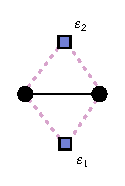
\includegraphics[scale=1.25]{figures/results/clusters/1D_2s_2b_cluster.pdf}
        \column{0.6\linewidth}
        \begin{figure}
            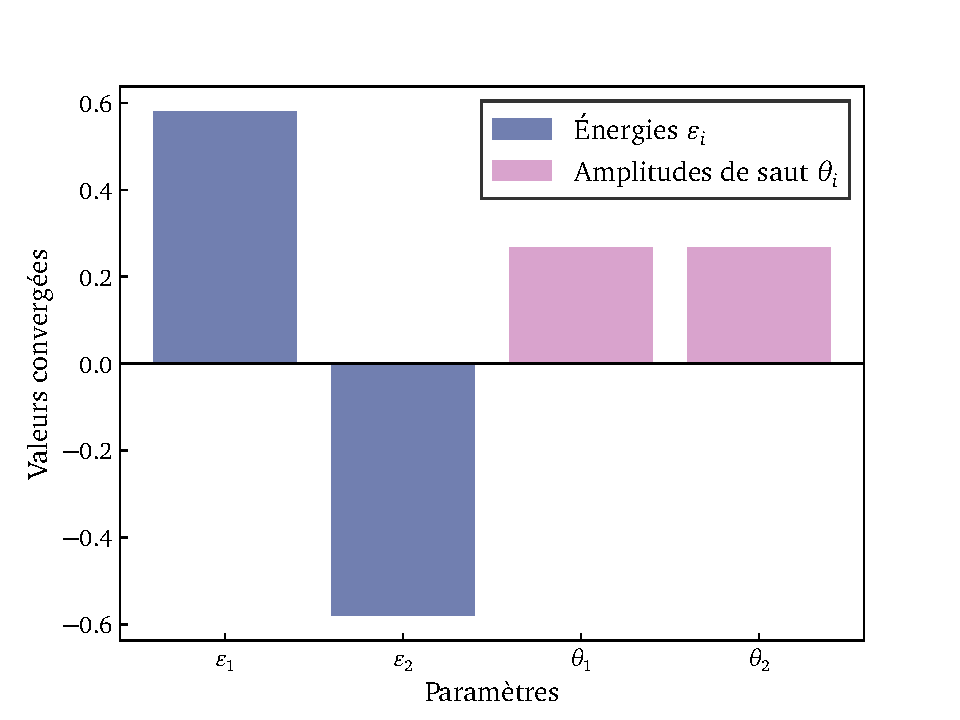
\includegraphics[scale=0.45]{figures/results/graphs/1D_2s_2b.pdf}
            \caption{Paramètres de bain d'un amas de deux sites réels lié à 2 sites de bain.}
            \label{fig: simu_2s_2b}
        \end{figure}
    \end{columns}
\end{frame}

\begin{frame}
    \frametitle{Résultats - CDMFT conventionnelle}
    \framesubtitle{Amas de 2 sites avec 4 sites de bain}
    \begin{columns}
        \column{0.4\linewidth}
        \centering
        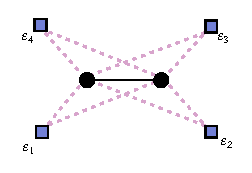
\includegraphics[scale=1.1]{figures/results/clusters/1D_2s_4b_cluster.pdf}
        \column{0.6\linewidth}
        \begin{figure}
            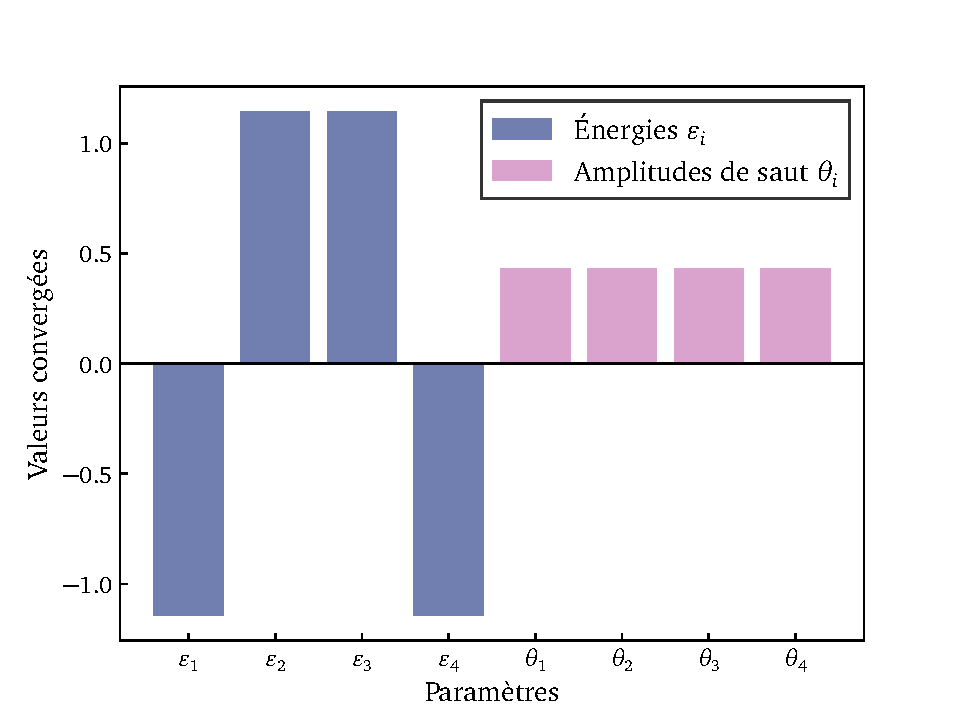
\includegraphics[scale=0.45]{figures/results/graphs/1D_2s_4b.pdf}
            \caption{Paramètres de bain d'un amas de deux sites réels lié à 4 sites de bain.}
            \label{fig: simu_2s_4b}
        \end{figure}
    \end{columns}
\end{frame}

\begin{frame}
    \frametitle{Résultats - CDMFT à bains virtuels}
    \framesubtitle{Amas de 2 sites avec 2 sites de bains par sous-bain}
    \begin{columns}
        \column{0.4\linewidth}
        \centering
        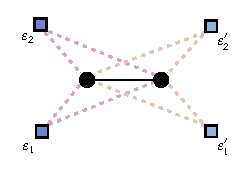
\includegraphics[scale=1.1]{figures/results/clusters/1D_2s_2vb_cluster.pdf}
        \column{0.6\linewidth}
        \begin{figure}
            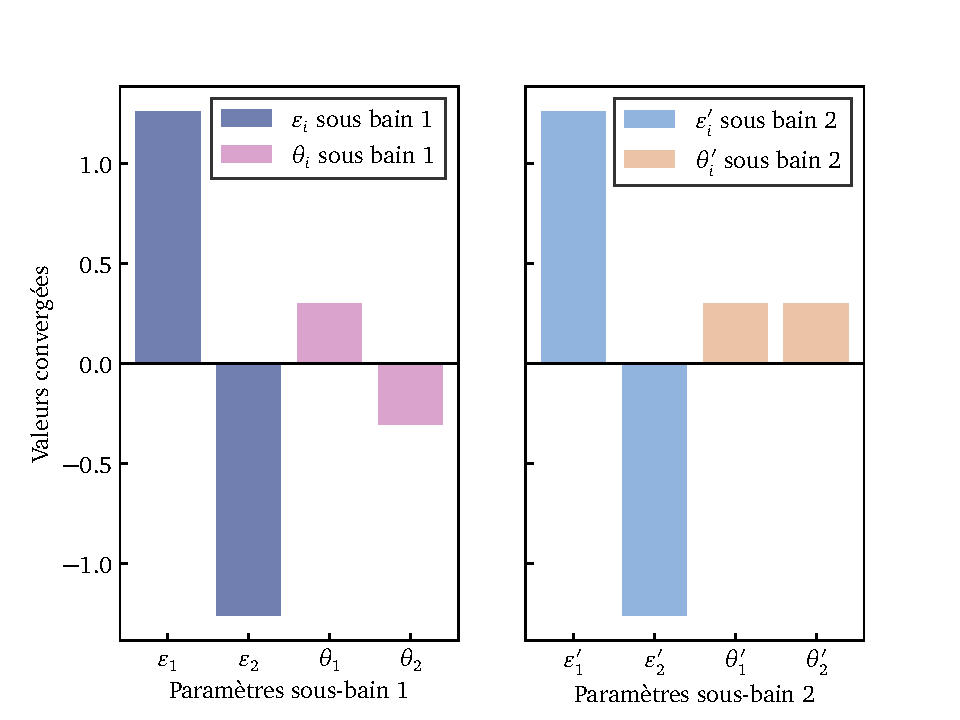
\includegraphics[scale=0.45]{figures/results/graphs/1D_2s_2vb.pdf}
            \caption{Paramètres de bain d'un amas de deux sites réels lié à 2 sous-bains de 2 sites.}
            \label{fig: simu_2s_2vb}
        \end{figure}
    \end{columns}
\end{frame}

\begin{frame}
    \frametitle{Résultats - CDMFT à bains virtuels}
    \framesubtitle{Amas de 2 sites avec 4 sites de bains par sous-bain}
    \begin{columns}
        \column{0.4\linewidth}
        \centering
        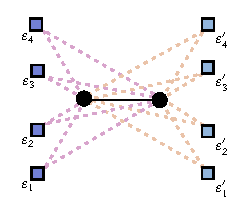
\includegraphics[scale=0.9]{figures/results/clusters/1D_2s_4vb_cluster.pdf}
        \column{0.6\linewidth}
        \begin{figure}
            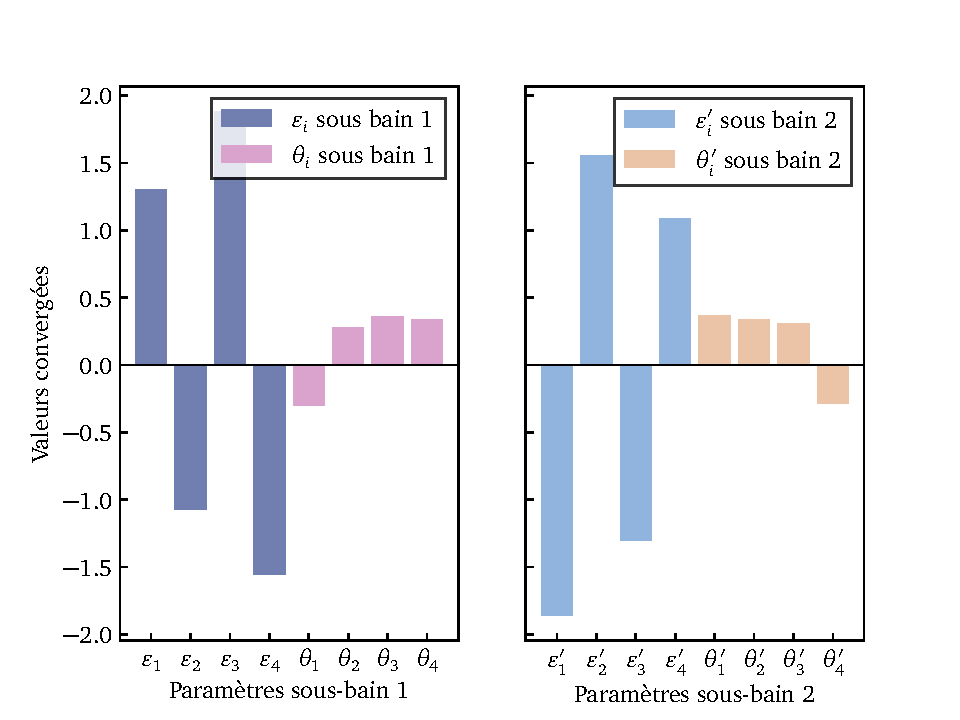
\includegraphics[scale=0.45]{figures/results/graphs/1D_2s_4vb.pdf}
            \caption{Paramètres de bain d'un amas de deux sites réels lié à 2 sous-bains de 4 sites.}
            \label{fig: simu_2s_4vb}
        \end{figure}
    \end{columns}
\end{frame}
